\documentclass[a4paper,12pt]{report}
%\usepackage[czech]{babel}      % česky psaná práce
\usepackage[T1]{fontenc}
\usepackage[utf8]{inputenc}  % vstupní znaková sada: Windows 1250
%\usepackage[latin2]{inputenc}  % vstupní znaková sada: ISO Latin 2

\usepackage{amsmath} % balíček pro pokročilou matem. sazbu
\usepackage{epsfig} % balíčky pro vkládání grafických souborů typu EPS
\usepackage{graphicx} % balíček pro vložení grafických souborů typu JPG -- přeložte pomocí PDFtex!
\usepackage{color}
\usepackage[table]{xcolor}
%\usepackage{fancybox} % umožňuje pokročilé rámečkování :-)
%\usepackage{index} % nutno použít v případě tvorby rejstříku balíčkem makeindex
\usepackage{tabularx}
\usepackage{float}

%\newindex{default}{idx}{ind}{Rejstřík} % zavádí rejstřík v případě použití balíku index

% na generovani textu
\usepackage[english]{babel}
\usepackage{blindtext}
\usepackage{lipsum}

\usepackage{wrapfig}
\usepackage{todonotes}
\usepackage{menukeys}


\usepackage{hyperref}
\hypersetup{pdftitle=Design of an Information System for Support of Forensic Audit}
\hypersetup{pdfauthor=Edita Pešková}


\hypersetup{
    colorlinks,
    citecolor=blue,
    filecolor=blue,
    linkcolor=blue,
    urlcolor=blue
}

%odstraneni cislovani od 0


\oddsidemargin=10mm   % levý okraj větší (kvůli vazbě)
\topmargin=-15mm      % horní okraj trochu menší
\textwidth=150mm      % šířka textu na stránce
\textheight=240mm     % "výška" textu na stránce


\pagenumbering{arabic} % číslování stránek arabskými číslicemi
\pagestyle{plain}      % stránky číslované dole uprostřed
\parindent=0pt % odsazení 1. řádku odstavce
\parskip=7pt   % mezera mezi odstavci
\frenchspacing % aktivuje použití některých českých typografických pravidel

% definice makra pro české uvozovky:
\def\bq{\mbox{\kern.1ex\protect\raisebox{-1.3ex}[0pt][0pt]{''}\kern-.1ex}}
\def\eq{\mbox{\kern-.1ex``\kern.1ex}}
\def\ifundefined#1{\expandafter\ifx\csname#1\endcsname\relax }%
\ifundefined{uv}%
        \gdef\uv#1{\bq #1\eq}
\fi
% konec .... použití makra pro psaní český uvozovek: \uv{text uvnitř uvozovek}



%=========================================================



%\newcommand{\todo}
%{{\it
%}}
%\newcommand{\todo}
%{{\it \color{magenta}
%\ldots TODO \ldots
%}}
%\newcommand{\name}
%{{\textit
%}}
%

\def\name{\textit}

%=========================================================


%%%%%%%%%%%%%%%%%%%%%% zde jsou zavedeny některé "konstanty" - můžete, resp. musíte je ZMĚNIT %%%%%%%%%%%%%%%%%%%%%%
\newcommand{\cvut}{Czech Technical University}
\newcommand{\fjfi}{Faculty of Nuclear Sciences and Physical Engineering}
\newcommand{\kse}{Department of Mathematics}
\newcommand{\obor}{Applied Information Technology}
\newcommand{\zamereni}{}

\newcommand{\nazevcz}{Návrh informačního systému pro podporu forenzního auditu}        % zde VYPLŇTE český název práce (přesně podle zadání!)
\newcommand{\nazeven}{Design of an Information System for Support of Forensic Audit}     % zde VYPLŇTE anglický název práce (přesně podle zadání!)
\newcommand{\autor}{Edita Pešková}           % zde VYPLŇTE své jméno a příjmení
\newcommand{\rok}{2015}                % zde VYPLŇTE rok odevzdání, např. 2006
\newcommand{\vedouci}{Mgr. Karel Macek, Ph.D.}         % zde VYPLŇTE jméno a příjmení vedoucího práce, včetně titulů
                                                               % např. Doc. Ing. Ivo Malý, Ph.D.
\newcommand{\pracovisteVed}{Oddělení ekonometrie, Ústav teorie informace a automatizace} % zde VYPLŇTE pracoviště vedoucího práce, je-li jiné než KSE FJFI ČVUT

\newcommand{\konzultant}{---} % POKUD MÁTE určeného konzultanta, NAPIŠTE jeho jméno a příjmení
\newcommand{\pracovisteKonz}{} % POKUD MÁTE konzultanta, NAPIŠTE jeho pracoviště


\newcommand{\klicova}{Forenzní audit, Vyšetřování, Návrh systému, Databáze, Sběr dat}  
\newcommand{\keyword}{Forensic audit, Investigation, System design, Database, Data collection}    
\newcommand{\abstrCZ}{%zde NAPIŠTE abstrakt v češtině
\textcolor{red}{Tato bakalářská práce předkládá návrh systému a naznačuje požadavky, které jsou potřebné aby byl popsán smysl a cíle technik digitálního forenzního vyšetřování, vykonávaných forenzními auditory, účetními a inpektory firem. Pomocí různorodých postupů, nástrojů a technik rozpoznáváme v jakých případech mohou nástroje forenzního auditu poskytnout auditorům potřebné informace k~provedení forenzního auditu. Bakalářská práce představuje požadavky, které musí splňovat vlastní informační systém použitelný pro podporu vyšetřování a také poskytuje detailní návrh tohoto systému. 
} }
\newcommand{\abstrEN}{     %              zde NAPIŠTE abstrakt v angličtině
\textcolor{red}{This bachelor project proposes a system design and suggests requirements that are needed in order to describe the purpose and goals of the digital forensic investigation techniques carried out by the forensic auditors, accountants and examiners of companies. Using various procedures, tools and techniques we identify where the forensic audit tools and the system can provide the auditors necessary information to carry out forensic audit. This bachelor thesis provides requirements that our own information system usable to support forensic audit must follow and also provides a detailed design of this system. 
}}
\begin{document}


%%%%%%%%%%%%%%%%%%%%%% 1. strana -- na následujících 30 řádků NESAHEJTE!!!  Generuje se AUTOMATICKY %%%%%%%%%%%%%%%%%%%%%%
\thispagestyle{empty}

\begin{center}
    {\Large \bf \cvut\\[2mm] \fjfi }
    \vspace{10mm}

    \begin{tabular}{c}
    {\bf \kse}\\
    {\bf Branch of Studies: \obor}\\
    %{\bf Zaměření: \zamereni}
    \end{tabular}

   % logo CVUT -- pokud jej nechcete použít, zakomentujte následující řádek a odkomentujte řádek pod ním:
   \vspace{10mm} \epsfysize=25mm \epsffile{cvut-logo-bw.eps} \vspace{15mm}
   \vspace{50mm}

   %\Huge \bf \nazevcz \par \nazeven\par}
   {\Huge \bf \nazeven\par}

   \vspace{15mm}
   {\Large Bachelor's Degree Project}

   \vfill
   {\large
    \begin{tabular}{rl}
    Author: & \autor\\
    Adviser: & \vedouci\\
    Language Adviser: & Mgr. Hana Čápová\\
    Academic Year: & \rok
    \end{tabular}
   }
\end{center}



%%%%%%%%%%%%%%%%%%%%%% 2. strana: zadání práce  %%%%%%%%%%%%%%%%%%%%%%
%%%%%%%%%%%%%%%%%%%%%%            Před svázáním namísto této strany VLOŽÍTE zadání podepsané děkanem!
\newpage  % SEM NESAHEJTE!
\thispagestyle{empty} Před svázáním místo téhle stránky \fbox{vložíte zadání práce} s podpisem
děkana (bude to jediný oboustranný list ve Vaší práci) !!!!



%%%%%%%%%%%%%%%%%%%%%% 3. strana: prohlášení -- ŽENY UPRAVÍ minulý čas sloves %%%%%%%%%%%%%%%%%%%%%%
\newpage % SEM NESAHEJTE!
\thispagestyle{empty}  % SEM NESAHEJTE!

~ % SEM NESAHEJTE!
\vfill % prázdné místo. SEM NESAHEJTE!

{\bf Declaration} % SEM NESAHEJTE!

\vspace{0.5cm} % vertikální mezera. SEM NESAHEJTE!
I declare that this Bachelor Project is all my own work and I have cited all sources I have used in the bibliography.

\vspace{5mm}In Prague ......................\hfill   % SEM NESAHEJTE!
    \begin{tabular}{c}                               % SEM NESAHEJTE!
    ........................................\\       % SEM NESAHEJTE!
    \autor                                           % SEM NESAHEJTE!
    \end{tabular}                                    % SEM NESAHEJTE!



%%%%%%%%%%%%%%%%%%%%%% 4. strana: poděkování -- UPRAVTE JMÉNO, resp. tuto stránku celou VYMAŽTE %%%%%%%%%%%%%%%%%%%%%%
%%%%%%%%%%%%%%%%%%%%%%                           (poděkování nemusí být uvedeno vůbec)
\newpage
\thispagestyle{empty}

~
\vfill % prázdné místo

{\bf Acknowledgements }

\vspace{5mm} % vertikální mezera
%Děkuji \todo %Ing. Eleonoře Krtečkové, Ph.D. za vedení mé bakalářské práce a za podnětné návrhy, které ji obohatily.

I wish to thank to my supervisor for his inspiring feedback, my family for their patience and support in my studies and anyone who encouraged me in this project. 

\begin{flushright}
\autor
\end{flushright}  % <------- tady končí stránka s poděkováním



%%%%%%%%%%%%%%%%%%%%%% 5. strana: abstrakt atp. Je generován AUTOMATICKY podle údajů na začátku souboru) %%%%%%%%%%%%%%%%%
\newpage   % SEM NESAHEJTE!
\thispagestyle{empty}   % SEM NESAHEJTE!

% příprava:    (na následujících 8 řádků NESAHEJTE!)
\newbox\odstavecbox
\newlength\vyskaodstavce
\newcommand\odstavec[2]{%
    \setbox\odstavecbox=\hbox{%
         \parbox[t]{#1}{#2\vrule width 0pt depth 4pt}}%
    \global\vyskaodstavce=\dp\odstavecbox
    \box\odstavecbox}
\newcommand{\delka}{120mm} % šířka textů ve 2. sloupci tabulky

% použití přípravy:    % dovnitř "tabular" vůbec NESAHEJTE!
\begin{tabular}{ll}
  {\em Název práce:} & ~ \\
  \multicolumn{2}{l}{\odstavec{\textwidth}{\bf \nazevcz}} \\[5mm]
  {\em Autor:} & \autor \\[5mm]
  {\em Obor:} & \obor \\
  {\em Druh práce:} & Bakalářská práce \\[5mm]
  {\em Vedoucí práce:} & \odstavec{\delka}{\vedouci \\ \pracovisteVed} \\[5mm]
  {\em Konzultant:} & \odstavec{\delka}{\konzultant \\ \pracovisteKonz} \\[5mm]
  \multicolumn{2}{l}{\odstavec{\textwidth}{{\em Abstrakt:} ~ \abstrCZ \\ }} \\[5mm]
  {\em Klíčová slova:} & \odstavec{\delka}{\klicova} \\[20mm]

  {\em Title:} & ~\\
  \multicolumn{2}{l}{\odstavec{\textwidth}{\bf \nazeven}}\\[5mm]
  {\em Author:} & \autor \\[5mm]
  \multicolumn{2}{l}{\odstavec{\textwidth}{{\em Abstract:} ~ \abstrEN \\ }} \\[5mm]
  {\em Key words:} & \odstavec{\delka}{\keyword}
\end{tabular}



%%%%%%%%%%%%%%%%%%%%%% 6. strana: obsah práce ... je generován AUTOMATICKY %%%%%%%%%%%%%%%%%%%%%%
\newpage  % SEM NESAHEJTE!
\setcounter{page}{1}
\tableofcontents % SEM NESAHEJTE!

%%%%%%%%%%%%%%%%%%%%%%  7.strana: zde začíná SAMOTNÁ PRÁCE  %%%%%%%%%%%%%%%%%%%%%%%%%%%%%%%%%%%%%%%%%%%%
%                                 - text se vkládá Z EXTERNÍCH SOUBORŮ
%                                   (můžete ho také napsat přímo sem => smažte každé \input{...})
\newpage % SEM NESAHEJTE!

\newcommand{\komentar}[1]{{\leavevmode\color[rgb]{1.0, 0.13, 0.32}#1}}
\newcommand{\sediva}[1]{{\leavevmode\color[rgb]{0.5, 0.5, 0.5}#1}}

\setcounter{chapter}{0}
\setcounter{section}{1}

\addcontentsline{toc}{chapter}{Introduction} % SEM NESAHEJTE!
\chapter*{Introduction} \label{Introduction}
% !TeX spellcheck = en_US
%uvedes problem, popises ho, proc je to problem, proc to resime, v cem nam to pomuze, kdyz ho vyresime; 
%a zminis, ze tato prace se snazi tento problem resit (ale uz ne moc jak).


%This bachelor project is concerned with the usage of software solutions in the field of forensic audit. 

%he basic definition of forensic audit is an assessment of a company's or individuals financial data or utilization as evidence in court. This procedure can be used with a specific end goal to indict for extortion, financial issues or embezzlement. 
%


%Forensic audit concentrates on the investigative procedure and its diverse stages and are represented by instinctive methodologies. This project proposes a dynamic model of the digital forensic model in the light of a new flow-based detailed system. It is demonstrated in samples that the technique can consistently indicate the forensic process in different stages and crosswise over portions. It likewise gives more correct depiction where things like data and confirmation are isolated into diverse streams of flow.


%\paragraph{Project Rationale}
There are two main areas in this project. At first the field of forensic audit and its frequently recurring processes are introduced. Secondly an information system for support of forensic audit is discussed and designed. The result of this project is a guide for a programmer to help easily implement a system usable in the field of forensic audit.


In the first part of this bachelor project we get to know the whole branch of forensic audit together with some of the issues that are commonly appearing while conducting the job of a forensic auditor. Next we propose several methods of forensic audit and we try to analyze whether a computer support is appropriate to be considered. Examples of available software solutions for selected cases are also offered. With regard to introduced methodology, we describe the requirements on our own system that could be helpful in the execution of forensic audit. In the following section a design of the new application is systematically described. UML diagrams are used to clarify the system design. A discussion about technologies to be used for implementation is provided in the end of this project. Final chapter is dedicated to a conclusion. 



\sediva{ \blindtext}
\komentar{ klicova slova: forenzni audit, unik penez, prosetreni spolecnosti, vyhledavani dukazu, pocitacova podpora, aplikace podporujici forenzni audit, vizualizace procesu vysetrovani, report o vysetrovanem pripadu, metodika forenzniho auditu, navrh informacniho systemu, ... }





















 



\addcontentsline{toc}{chapter}{Forensic audit and its computer support}
\chapter{Forensic audit and its computer support}


\komentar{na zacatek shrnout co vsechno obsahuje tato kapitola}


\section{Forensic audit}
\subsection*{Definition}
\komentar{- zde v hrubych rysech jak to probiha (to co uz mam sem patri), na zaklade toho, co jsem zjistila FA funguje takto:...}




\komentar{
\subsection*{use case diagram}
Velky obrazek vsech zainteresovanych stran - f.auditor, datovy analytik pro FA, zakaznik (zadavatel, materska spolecnost)
}





\addcontentsline{toc}{chapter}{Original methodology for the (computer aided) forensic audit}
\chapter{Original methodology for the (computer aided) forensic audit}
\komentar{Jsem si vedoma, ze jsem clovek, ktery to nikdy nedelal (= omezena znalost).
Toto je jak to chapu. Toto neni jak by to nekdo mel delat. Toto je seriozni pokus popsat proces forenzniho auditu.
PROCESNI DIAGRAMY!!!

vystupem = okomentovany obrazek, ktery dava hlavu a patu

a Use case diagrammem pak kontaktovat praxi

}

\chapter{Design of an information system for support of forensic audit}
\komentar{
vsechno o tom systemu jako takovem, ale tak, aby to navazovalo na predchozi...?

prostredi webu + silne zabezpeceni, reporty, export, pdf\\
maly informativni obrazek, ktery poskytne uzivateli informaci o tom, co se stalo\\
! pripojit pripady uziti vcetne zavislosti\\

jedna se o aplikaci, ktera provazi celym projektem (zadanim) forenzniho auditu. sice existuji i jiny nastroje pro podporu takovychto projektu, ale projekt ma useky a nam jde o integraci porizenych vysledku


}

\chapter{Discussion}
\komentar{
	\section{Further improvements}
\begin{itemize}
	\item pokryt dalsi administrativni casti (zacatek, konec)
	\item detailnejsi navrh a implementace
	\item detailnejsi osetreni rizik
	\item zamysleni nad sdilenim zkusenosti (duvernost vs. rust expertyzy auditorske spolecnosti)
	\item vyuziti mimo FA - jina administrativa + moduly pro vyuziti policii / soudy
\end{itemize}
	
	
	pouzitelne technologie!
}



%\chapter*{Introduction} \label{Introduction}
% !TeX spellcheck = en_US
%uvedes problem, popises ho, proc je to problem, proc to resime, v cem nam to pomuze, kdyz ho vyresime; 
%a zminis, ze tato prace se snazi tento problem resit (ale uz ne moc jak).


%This bachelor project is concerned with the usage of software solutions in the field of forensic audit. 

%he basic definition of forensic audit is an assessment of a company's or individuals financial data or utilization as evidence in court. This procedure can be used with a specific end goal to indict for extortion, financial issues or embezzlement. 
%


%Forensic audit concentrates on the investigative procedure and its diverse stages and are represented by instinctive methodologies. This project proposes a dynamic model of the digital forensic model in the light of a new flow-based detailed system. It is demonstrated in samples that the technique can consistently indicate the forensic process in different stages and crosswise over portions. It likewise gives more correct depiction where things like data and confirmation are isolated into diverse streams of flow.


%\paragraph{Project Rationale}
There are two main areas in this project. At first the field of forensic audit and its frequently recurring processes are introduced. Secondly an information system for support of forensic audit is discussed and designed. The result of this project is a guide for a programmer to help easily implement a system usable in the field of forensic audit.


In the first part of this bachelor project we get to know the whole branch of forensic audit together with some of the issues that are commonly appearing while conducting the job of a forensic auditor. Next we propose several methods of forensic audit and we try to analyze whether a computer support is appropriate to be considered. Examples of available software solutions for selected cases are also offered. With regard to introduced methodology, we describe the requirements on our own system that could be helpful in the execution of forensic audit. In the following section a design of the new application is systematically described. UML diagrams are used to clarify the system design. A discussion about technologies to be used for implementation is provided in the end of this project. Final chapter is dedicated to a conclusion. 



\sediva{ \blindtext}
\komentar{ klicova slova: forenzni audit, unik penez, prosetreni spolecnosti, vyhledavani dukazu, pocitacova podpora, aplikace podporujici forenzni audit, vizualizace procesu vysetrovani, report o vysetrovanem pripadu, metodika forenzniho auditu, navrh informacniho systemu, ... }






















%\chapter*{Overview} \addcontentsline{toc}{chapter}{Overview} % SEM NESAHEJTE!
%% !TeX spellcheck = en_US 
\chapter{Overview} \label{Overview}


This chapter focuses on the review of the work practiced in this field and the issues associated with the existing forensic investigation systems. It also discusses the purposes, aims and use of a digital forensic investigation system that we will be designing later on. 

Forensic audit is a specialization within a field of accounting that examines and evaluates evidence concerning unproven statements for use as evidence in court. Forensic audit is usually used to investigate the particular crime that has happened. When the exact sequence of events that has led to the crime is investigated and found, it serves as a clear and valid evidence for the hypothesis. The person responsible for the crime is also being searched for, although there is another case when forensic audit is used. This situation occurs when it is not known whether any crime has been committed. Then forensic audit will be conducted to detect, whether in a certain vast company or project any crime has been committed. These case hypotheses are created and then confirmed or disproved according to well examined facts.

Forensic audit therefore deals with assessment of companies or individual's financial data and performance for using it as evidence. It can be used with a specific end goal to investigate the misuse and financial issues of the company. The forensic audits will concentrate on the investigative procedure and its diverse stages to represent them by instinctive methodologies. This bachelor project proposes a design of an information system that can be helpful in one of the stages of forensic audit. 



Digital PC legal forensics that is characterized as expository and investigative strategy is used for safeguarding, proof recognizing, extraction, documentation, investigation and translation of PC media. In this bachelor project we make use of the digital forensics as it provides us the source of information that we display later on. Forensic investigation focus on handling of the criminal cases identified with PCs and systems and also carry out inward corporate examinations and disciplinary inquiries. It may include the obtaining and examination of advanced proof, verification of records, ID of sources and suspects, etc. 


Targeting on a forensic investigation requires going through a few stages. Models of computerized forensics will be described in order to comprehend the logical evidence of the field \cite{3}. As indicated by \cite{4}, such investigation will have an immediate effect on:

\begin{itemize}
\item Anticipation of further malicious instances;
\item Modification of current prevention systems;
\item Enhanced principles for corporate security experts;
\item Expanded consciousness of current vulnerabilities and preventive measures.
\end{itemize}


\section{Review of forensic investigation} 
With the advent of digital revolution in the second half of 90s, the lifestyle of billions of people has changed significantly. In the beginning, all these innovations seemed to be something just to have fun with, but quickly people begun to use the Internet, mobile phones, and other various digital devices in both their professional and personal lives. These technologies have become an indispensable part of everyday life. 

To highlight expectations in this project, we specify here a couple of samples as reviewed in that are specifically identified with our technique of demonstrating. “Pollitt” \cite{3} distinguished four stages in computerized forensic scene investigation, that take after: securing, distinguishing proof, assessment, and affirmation of confirmation, and further portrayed suitability of proof. “The National Institute of Standards and Technology (NIST)” \cite{20} characterizes the fundamental measurable process as following: 

\paragraph{Accumulation:} 
The main stage in the process is to recognize, mark, record, and gain information from the conceivable sources of pertinent information. 

\paragraph{Examination:}
Examinations include forensically preparing a lot of gathered information utilizing a blend of computerized and manual systems to survey and concentrate information specifically compelling. 

\paragraph{Investigation:}
The following period of the procedure is to investigate the consequences of the examination, using legitimately reasonable routines and systems, to infer helpful data that addresses the inquiries that were the impulse for performing the accumulation and examination. 


\paragraph{Reporting:}
The last stage is reporting the consequences of the investigation, which may incorporate depicting the activities utilized, clarifying how devices and methods were chosen, figuring out what different activities should be performed and giving proposals ti change to approaches, rules, techniques, apparatuses, and different parts of the measurable procedure. 

%!!!!CITACE %   Other proposed models incorporate those depicted by Reith, Carr and Gunsch \cite{5}, Carrier and Spafford \cite{6}, Ademu, Imafidon, and Prestonn \cite{8}, and Ciardhuain \cite{7}.


The quantity of different data stored in a digital form is constantly increasing. These data are, for example emails, digital photos, instant messaging history, or phone books.

Our societies have been transforming some traditional crimes, particularly those concerning finance and commerce. For this reason, the importance of an analysis of digital and computer devices has emerged. The field of computer forensic have been created to respond to the needs of the law enforcement and to discover all the digitally stored evidence.

\section{Issues of digital forensic investigation}
As per Tanner and Dampier, digital forensic investigations are turning out to be more unpredictable because of the expanding size of computerized storage. New methodologies for dealing with the digital forensic investigations must be created. In particular, what is needed is to create examination benchmarks and to give structure to PC measurable examinations, furthermore, to capture the tools included in advanced forensic scene investigation \cite{5}.


As indicated by Kohn, Eloff, and Olivier \cite{6}, the majority of the demonstrating representations for measurable examinations found in the present writing  of 2003 are made in a fairly casual and instinctive way". Likewise, "It can be securely said that current models are basically unplanned and should be completed in the specific space" \cite{4}. This bachelor project proposes a conceptual model of the advanced legal strategy taking into account another flow based determination technique that has been used as a part of a few examinations areas.



%\section{Clarification of terms} %upresneni pojmu 

%To clearly understand the issue, it is appropriate to clarify all terms related to the project. 
%Although all of them might not be needed, they are all in a manner associated to the subject, 
%therefore they are worth mentioning.

\subsection{Purpose of forensic audit} 
The purpose of forensic audit is to use accounting procedures to collect evidence for the prosecution or investigation of financial crimes such as theft or fraud. Forensic audits may be conducted to determine if any wrongdoing occurred, or to gather materials for the case against an alleged criminal \cite{x1}.
%Read more: http://www.investorwords.com/16445/forensic_audit.html#ixzz3SFC3Lqlf

%Forensic audit is a specialization within the field of accounting that examines and evaluates evidence concerning unproven statements for use as evidence in court.

Forensic audit is usually used to investigate the particular crime that has happened. In this case the exact sequence of events that has lead to the crime is investigated and when found, it serves as a clear and valid evidence for the hypothesis. The person responsible for the crime is also being searched for. However, there is another case when forensic audit is used. This situation occurs when it is not known whether any crime has been committed. Then forensic audit is conducted to detect whether it is the case or not. These cases usually occur in a vast company or project. In these cases hypotheses are created and then confirmed or disproved according to well examined facts.

\begin{itemize}
\item\textbf{Computer Forensics} is used for investigation of situations where there is a computer-based digital or electronic evidence of a crime or a suspicious behavior. The crime or behavior itself may be of any type not only involving computers.


\item\textbf{Mobile Forensics} is a discipline that primarily analyses mobile applications such as smart phones or GPS navigation systems. 


\item\textbf{Digital Forensics}  is a specialization of forensic science that processes material found in digital devices to support or displace a hypothesis before court.


"It is asserted that digital forensics is a procedure that can be demonstrated with some sensibly settled stages" \cite{4}. Most proposed legal models have concentrated on "the investigative procedure and the distinctive stages that they tend to the quality of an examination and the components and usefulness of tools and the solid standards of an examination.% \cite{5}. ??
\end{itemize}


To highlight expectations in this project, we specify here a couple of examples as reviewed in \cite{3} that are specifically identified with our technique of demonstrating. Pollitt \cite{3} distinguished four stages in computerized forensic scene investigation, that take after: securing, distinguishing proof, assessment, and affirmation of confirmation, and further portrayed suitability of proof. Bearer \cite{1} sketched out layers of deliberation of legal examination where every layer has two inputs and two yields. The National Institute of Standards and Technology (NIST) \cite{3} characterize the fundamental measurable process as following:

\paragraph{Accumulation:} 
The main stage in the process is to recognize, mark, record, and gain information from the conceivable sources of pertinent information. 

\paragraph{Examination:}
Examinations include forensically preparing a lot of gathered information utilizing a blend of computerized and manual systems to survey and concentrate information specifically compelling. 

\paragraph{Investigation:}
The following period of the procedure is to investigate the consequences of the examination, using legitimately reasonable routines and systems, to infer helpful data that addresses the inquiries that were the impulse for performing the accumulation and examination. 


\paragraph{Reporting:}
The last stage is reporting the consequences of the investigation, which may incorporate depicting the activities utilized, clarifying how devices and methods were chosen, figuring out what different activities should be performed and giving proposals ti change to approaches, rules, techniques, apparatuses, and different parts of the measurable procedure. 

Other proposed models incorporate those depicted by Reith, Carr and Gunsch \cite{5}, Carrier and Spafford \cite{6}, Ademu, Imafidon, and Prestonn \cite{8}, and Ciardhuain \cite{7}.

To keep this bachelor project independent, the following segment surveys essential components of the model on which our technique for depicting forensic scene investigation examination is constructed. 

%\todo{} udelat v .ppt  a pridat sem hezky graf ukazujici, jake oblasti spadaji pod 
%forenzni audit a kde se nachazi dalsi terminy

%\section{Project schedule}
%To successfully complete the project it is essential to follow the points below. 
%\begin{itemize}
%\item Evaluate existing programs
%\item Specify requirements of suitable application
%\item Develop our own reasoned and systematic methodology and system design
%\item Develop a system design using UML diagrams
%\item Discuss suitable technology for application development
%\item Summarize
%\end{itemize}



\section{Aims of the project} %cile prace 

The aim of this bachelor project is to design a software application which would help in one of the final stages of the process of forensic audit. The software will be designed to visually demonstrate actions of subjects of the particular case. The design of the software will be described properly.



%\chapter*{Analysis}\addcontentsline{toc}{chapter}{Analysis}
%% !TeX spellcheck = en_US
\chapter{Analysis}\label{Analysis}

The motivation behind forensic auditing is to devise a system that is not only user friendly and easy to use but also serves the purpose to help auditors with an extensive range of investigation. The work comprises of an investigation in the fiscal matters of a unit and is frequently allied with examinations into suspected deceitful activity.

Forensic auditing covers an extensive range of accomplishments, with terminology not strictly well-defined in the regulatory guidance. Forensic accounting is used to describe the widespread range of investigative exertion that examiners may in practice be requested to implement. The work comprises of an investigation in the fiscal matters of a unit and is frequently allied with examinations into suspected deceitful activity. Forensic accounting analyzes the whole procedure of investigating a fiscal matter, together with hypothetically acting as an expert spectator if the fraud comes to court of justice. 

Though this bachelor project concentrates on investigations into suspected frauds, it is essential to be aware that the forensic accountants may be asked to consider also non-fraud circumstances.
%, like resolving of financial disputes relative to a business termination or matrimonial clashes under insurance claims.

The procedure of forensic accounting analyses as designated above contains the forensic investigation itself, which indicates the practical phases that the forensic accountant undertakes in order to collect evidence pertinent to the suspected deceitful activity. The investigation is expected to be related in many means to an audit of financial evidence, in that it must contain a development phase, a period when proof is collected, an appraisal procedure, and a specific report to the user. The ambition of the investigation, in the matter of a suspected fraud, will be to determine if a deception had truly taken place in order to classify those involved, to enumerate the fiscal expanse of the deception i.e. the monetary cost by the user, and to eventually present the outcomes to the client and possibly to the court. 


Finally, forensic auditing deals with precise procedures approved to create evidence. Audit procedures are used to classify and to gather proof of, for example, how long ago the fraud has been carried out, and how it was handled and covered by the perpetrators. Proof is gathered to support other matters that would be pertinent in the occasion of a lawsuit. 

Such matters could consist of: 
\begin{itemize}
\item the defendant's motivation and convenience to commit the fraud 
\item to see if the fraud contained collusion among certain defendants
\item any physical proof at the area of the crime or included in the documents 
\item remarks made by the examiner throughout interviews and at the moment of arresting 
\item efforts to abolish evidence.
\end{itemize}

\section{Types of investigation}

The forensic auditor could be demanded to examine various sorts of fraud. To analyze the extensive area of examinations that could be completed, these sorts of fraud can be classified into three categories. The first category containing frauds such as conflict of interest, extortion or bribery. Approximately one third of fraudulent activities is somehow connected to corruption.In the second category we can find acts of cash theft, fraudulent disbursement or misuse of assets. This category can be generally called asset misappropriation and activities related to it are actually the most common frauds. All financial statement frauds may be considered as the third separate category, including all the deliberate misinterpretation of financial reporting standards or manipulation with obligations to improve analyses of liquidity. 



\subsection{Asset misappropriation}
Clearly the most widely recognized frauds are those including resource misappropriations and there are various sorts of misrepresentation which fall into this classification. The basic element is the burglary of money or different resources from the organization, for instance: 

\begin{itemize}
\item Cash burglary – the taking of physical money, for instance insignificant amount of money, from the premises of an organization.
\item Fraudulent payment – organization trusts being utilized to make fake installments. Regular illustrations incorporate charging plans where installments are made to an imaginary supplier and finance plans where installments are made to invented workers that are frequently known as 'apparition representatives'.
\item Inventory replicas – the robbery of stock from the organization. 
\item Misuse of benefits – representatives utilizing organization resources for their own interest.
\end{itemize}


\subsection{Financial statement fraud}

This is deceitful money related reporting, and is a kind of misrepresentation that causes a material misquote in the budgetary proclamations. It can incorporate planned distortion of bookkeeping records; exclusion of exchanges, equalizations or exposures from the budgetary explanations; or the misuse of money-related reporting guidelines. This is regularly done with the goal of giving the budgetary proclamations a specific inclination, for instance covering liabilities to enhance any examination of liquidity.


\section{Conducting the investigation}

The procedure of directing a forensic examination is, from various perspectives, like the procedure of leading a review, however, with some extra contemplation. The different stages are precisely discussed below.

\subsection{Accepting the investigation}

The forensic accountant will at first contemplate whether the firm has essential aptitudes and knowledge to acknowledge the work. As forensic examinations are professional in nature, and the work entails definite learning of misrepresentation examination strategies and legitimate system, agents should likewise prepare meetings and cross examination systems, and consider how to keep up the secure upkeep of proof accumulated.

Extra contemplations incorporate regardless of whether the examination is being asked for by a review customer. In the event that it is, this suggests additional moral conversation starters, as the examining firm would be possibly be presented to self-audit, promotion and administration risks to objectivity . Unless strong shields are set up, the firm ought not to give review and measurable examination administrations to the same client. Business contemplations are additionally critical and a high charge level ought to be arranged to make up for the way of the work and the conceivable contribution of senior and experienced individuals from the firm in the examination.


\subsection {Planning the investigation}

The examining group should precisely contemplate what they are requested to accomplish and arrange their work consequently. The purpose of this examination will include: 

\begin{itemize}
\item Identifying the sort of misrepresentation that has been working, to what extent it has been working to, and how the work has been hidden.
\item Identifying the fraud(s) included.
\item Quantifying the budgetary trouble endured by the ordering party.
\item Gathering confirmation to be utilized as a part of court procedures. 
\item Providing advice to avoid the fraud to be repeated.
\end{itemize}


The agents ought to additionally consider the most ideal approach to assemble proof i.e. the utilization of PC assisted review procedures, for instance, it is exceptionally regular in extortion examinations.

\subsection{Gathering proof}

To assemble the proofs, the forensic auditor must comprehend what particular sort of fraud that has happened, and how it has been accomplished. The evidence ought to be strong and adequate enough to eventually identify the fraudsters, their plan of accomplishing the fraud and, and the sum of money lost due to the fraud. It is essential that forensic auditors are talented in gathering proof that is usable proof in a trial, and in keeping the evidence hidden until it is displayed in court. If any proof is uncertain, then it may be called into question in court, or even be forbidden. 

Forensic auditors must be aware that some of the material may be falsified on purpose, impaired or ruined by the suspect(s).

\section{Summary of Investigation techniques}

A forensic examination tends to be an extremely expert kind of engagement, which requires highly talented individuals who have knowledge of audit methods, technology and also law. 

There are various diverse kinds of fraud that a forensic auditor could be requested to research. The examination tends to eventually prompt legitimate procedures against one or a few individuals.

Forensic auditors must be prepared to demonstrate at the court how the examination has been  performed and how the proofs have been gathered. Forensic auditors should therefore get expert training in such matters to guarantee that their credibility and polished skill can't be undermined in the time of the legitimate procedure. To become familiar with the present circumstances, examinations of tools that are being used as a part of the procedure of forensic audit have been performed. 


\begin{itemize}
\item{Tools used in investigation:}
%\begin{itemize}
%\item Public Databases \cite{10}
%\item Secretary of State Websites
%\item Country Seat
%\item Corporate Records
%\item Internet
%\end{itemize}

\begin{itemize}
\item{Public Databases \cite{10}}
\begin{itemize}
\item Increasing number of vendors
\item Reliability of data
\item What type of data is available?
\end{itemize}

\item{Internet}
\begin{itemize}
\item Search Engines \cite{10}
\item News Sources/Newspapers
\item Telephone Numbers and Addresses
\item Maps
\item Legal Resources
\item Government Sites \cite{10}
\item Computer Forensics
\begin{itemize}
\item hard disk imaging
\item E-mail analysis
\item search for erased files
\item analyze use \& possible misuse
\item computer software to analyze data \cite{10}
\end{itemize}
\end{itemize}

\item{Physical}
\begin{itemize}
\item usually done by law enforcement or PI's
\item surveillance cameras
\item can also be used to verify addresses for vendors, employees, etc. \cite{10}
\end{itemize}


\item{Electronic}
\begin{itemize}
\item Internet surveillance
\item E-mail \cite{10}
\end{itemize}
\end{itemize}
\end{itemize}


Obtaining information from equipment may require diverse systems relying upon information state and the numerous conceivable stockpiling structures. 

PC media drives such as RAM, CDs, DVD and Mobile gadgets including telephones, PDAs, iPods, GPS Network Infrastructure, printers, servers, O/S, Active Directory (AD),  databases, Cloud, Apple, iCloud, MobileMe, Amazon S3, Google and cloud storage all analyze the conditions of the equipment and information before communicating.


In a perfect world equipment ought to be gathered "in-state" and transported to secured, "flawless" environment for investigation. Obtained equipment requires approval for fulfillment and accuracy like information acceptance.


%\todo %vyjadrit se k otazce pocitacove podpory konkretnich fazi prosetrovani... (splnit zadani BP)

%
%To get to know the current situation an investigation of programs that are being used in the 
%process of forensic audit have been performed. Although the original idea, what the perfect 
%forensic-audit tool should look like is quite simple, (it should be just one tool that does 
%everything) the reality is entirely different. There \todo {is a lot of} tools that can be used 
%for a great number of situations one can get into while conducting a forensic audit 
%investigation. Moreover, in each specific situation, there is also a variety of associated 
%technical parameters and technical parameter values, that, in fact, often answer the question, 
%whether an initial problem has its solution in using one or another tool. 

\section{Existing software}

The existing software in the market is either inefficient in terms of results or does not full fill the requirements for conducting proper evaluation. For this reason, Computer Forensic Tool Catalog has been created as an effective way of connecting practitioners to the tools they need. This catalog is available on the "National Institute of Standards and Technology" web pages \cite{10}. The information about forensic functionalities and associated technical parameters and their values can be provided by any vendor, in order to be integrated to the database. All tools are being reviewed before posting. This catalog can be considered rich in the database and it is also systematic and searchable. The only problem is it is not possible to select free tools only. This catalog can be recommended to any practitioner as a useful instrument for choosing suitable software for their situation. Although other lists of software can be found browsing the Internet, this one is reliable and provides the possibility of search in the tools according to technological needs.

The functionalities of the tools contained in the catalog are mostly usable in one of the first stages of forensic audit. This stage could also be called preparatory stage because the auditor is preparing background for the search for evidence. Documents and all possibly available data related to the studied case are being collected. Depending on the character of the case, data from various pieces of hardware can be collected. In some situations, if the tool is sophisticated enough, the following analysis of the data can be performed immediately within the same tool.

The functionality choices in the Computer Forensics Tool Catalog \cite{20}:

\begin{itemize}
\item Cloud Services
\item Deleted File Recovery
\item Disk Imaging
\item Email Parsing
\item File Carving
\item Forensics Boot Environment
\item Forensic Tool Suite (Mac Investigations)
\item Forensic Tool Suite (Windows Investigations)
\item GPS Forensics
\item Hardware Write Block
\item Hash Analysis
\item Image Analysis (Graphics Files)
\item Infotainment and Vehicle Forensics
\item Instant Messenger
\item Media Sanitization/Drive Re-use
\item Memory Capture and Analysis
\item Mobile Device Acquisition, Analysis and Triage
\item P2P Analysis
\item Password Recovery
\item Remote Capabilities / Remote Forensics
\item Social Media
\item Software Write Block
\item Steganalysis
\item String Search
\item Web Browser Forensics
\item Windows Registry Analysis
\end{itemize}



The work of the auditor usually starts by getting to know the situation because each case has its specific character. After that they need to collect all the hardware that holds important data and extract all the data stored in these devices. According to the type of device they may use proper software that is good for acquisition of the data stored.


%//pridat tabulku reprezentujici: platformy, cena, funkce(), specifika, reprezentace dat, jak moc jsou bezne vyuzivane

\section{Software analysis}
\paragraph{Quantative software}\label{qSW}

Specialized fraud identifying software is making a passage into the business, with extortion module discharges from both ACL and IDEA\textsuperscript{\textregistered}, extortion parts in SAS and SPSS, and a devoted extortion discovery program in Picalo. Programming organizations like ACL and IDEA\textsuperscript{\textregistered} give exercise manuals that can be utilized as a part of courses, however, these exercise manuals have couple of illustrations of direct misrepresentation recognition particularly with cutting edge procedures. Approaches like the theory testing methodology are an initial phase in giving procedure research, immense extra research—both observational and field—are expected to approve and augment the current ideas.

Quantative software organizations give complete preparing on measurable programming and systems. The two driving programming bundles are EnCase by Guidance Software and the Forensic Toolkit (FTK) by Access Data . These suites give shorter expectations to absorb information than past utilities and convey a more prominent number of experts to the field more rapidly. Both bundles give tasks positioned procedures to securing and illustrating forensic information.


Lately, Linux based apparatuses have been prevalent as free distinct options for the conventional suites. Helix, the Penguin Sleuth, and Security Tools Distribution are Linux dispersions that run specifically from CD, giving clean situations to seeking a PC without the requirement for cloning (Causey, 2005). These instruments boot a suspect PC straightforwardly to Linux and mount the client hard drives in read just mode, basically bypassing most passwords and security insurances. While Linux based instruments are more hard to use and do not have the same point of reference in court as EnCase and FTK, they have to be well known with a few evaluators.


%TODO: poradne popsat qSW

\paragraph{The R Project for Statistical Computing} 
R is mathematical software specialized in statistics. It concerns an open-source implementation of the S language, which is used by other professional statistical applications. It is a good choice in case that great amount of data needs to be processed because R is suited for large data sets.
%\cite{http://www.r-project.org/about.html}


\paragraph{Using SAS to evaluate risks }

Measurable packages like SAS and SPSS give full drifting modules to the intrigued inspector. Statement on Auditing Standards (SAS) and consideration of fraud in a financial statement audit requires inspectors to evaluate the risk that misrepresentation might physically misquote budgetary articulations. Regardless of SAS 99 being an imperative necessity towards expanded misrepresentation, a study by "Marczewski and Akers"\cite{21} uncovered that Certified Public Accountants (CPAs) do not envision that SAS 99 will generously expand review viability. Another study found that while SAS 99 expanded examiner obligation, most reviewers experienced issues recognizing the work and its risks.



\paragraph{SPSS for statistical and analytical services}

SPSS is one of the leading analytical instruments. It provides statistical and analytical services the abbreviation originally meant Statistical Package for the Social Sciences. This software supports areas of social survey and market research, predictive and advanced analytics, decision management and deployment or predictive solutions.

%\cite{http://www-01.ibm.com/common/ssi/cgi-bin/ssialias?infotype=PM&subtype=BR&appname=SWGE_YT_YV_USEN&htmlfid=YTB03015USEN&attachment=YTB03015USEN.PDF}

\paragraph{COFEE}
Useful tools for basic forensics are Microsoft's COFEE tools. They are a set of PC forensic and evaluating tools that Microsoft puts on a USB key and provides for law requirement. It is used in attempting to concentrate information from a PC. There was some apprehension that it was an "indirect access", however, individuals demanded it was no such thing, yet only a gathering of essential tools. Still, the this framework was advanced as being valuable for decoding passwords and examining a PC's information and web action that appeared to be alarming. If Microsoft was giving it out to law requirement, it appeared to be likely that others would have entry to it also.


%doplnit!
\paragraph{IDEA\textsuperscript{\textregistered}}
IDEA\textsuperscript{\textregistered} is an effective and easy to understand information investigation tool intended to help reviewers; bookkeepers and other account experts perform information examination rapidly to help enhance reviews and distinguish control breakdowns. It permits to dissect 100\% of the information to ensure information trustworthiness and gives simple investigation more that 100 major studied activities. 

At the point when the information originates from distinctive sources and in a mixed bag of configurations, information investigation can infrequently be a test. The capacity to import different information sets and represents it as if they were one that lets us to see the master plan. We have the capacity to recognize connections, examples and inconsistencies and additionally direct a far reaching examination of value-based information. 

Import Data from Practically Any Source IDEA\textsuperscript{\textregistered} permits us to rapidly import a boundless measure of records from for all intents and purposes of any source, including spreadsheet and \textbf{database programming}, mid-extent bookkeeping projects, ERP frameworks, legacy centralized servers, telecommunication switches, travel and costs applications, level and printed documents, for example, PDFs, plain content (.txt), and print-report (.prn) records. Rearranged analysis instead of programming macros can use more than 100 review particular undertakings that easily search for copies, identify dumps in numeric groupings, group information by classes and channel various lines and sections of data in seconds. IDEA\textsuperscript{\textregistered} permits us to record each investigative step and reuse for future utilization, through a graphical interchange and customized interface. 

\paragraph{Microsoft Analytics Services}
Procedures utilized for misrepresentation discovery fall into two essential classes: factual systems and computerized reasoning. Examples of measurable information examination methods are: 

\begin{itemize}
\item Data preprocessing strategies for discovery, acceptance, slip adjustment, and topping of missing or off base information.
\item Calculation of different factual parameters, for example, midpoints, quintiles, execution measurements, lihelihood circulations. For instance the midpoints may incorporate normal length of call, normal number of calls every month and normal defers in bill installment.
\item Models and likelihood dispersions of different business exercises either regarding different parameters or likelihood circulations.
\item Computing client profiles.
\item Time-arrangement investigation of time-ward information.
\item Clustering and grouping to discover examples and relationship among gatherings of information.
\item Matching calculations to recognize abnormalities in the conduct of exchanges or clients when contrasted with already known models and profiles. Methods are likewise expected to dispose of false alerts, assessment chances, and foresee eventual fate of current exchanges or clients. % \todo cite.
\end{itemize}

Some measurable bookkeepers work in criminological investigation which is the acquisition and examination of electronic information to reproduce, distinguish, or generally bolster a case of monetary misrepresentation. The fundamental strides in criminological examination are (a) information gathering, (b) information planning, (c) information investigation, and (d) reporting \cite{16}.Case in point, forensic examination may be utilized to audit a representative's obtaining card action on evaluate whether any of the purchases were occupied or divertible for individual utilization. Forensic examination may be utilized to survey the invoicing action for merchant to distinguish imaginary sellers, and these systems may likewise be utilized by franchisor to recognize deceitful or mistaken deals reports by the franchise in a franchising situation.

In the next step the reviewer needs to process picked up information to have capacity to some criminological bookkeepers and spend significant time in legal investigation which is the acquisition and examination of electronic information to remake, distinguish, or generally bolster a case of budgetary extortion. The principle ventures in legal investigation are (a) information gathering, (b) information arrangement, (c) information examination, and (d) reporting. For instance, legal examination may be utilised to survey a worker's buying card action to evaluate whether any of the buys were occupied or divertible for individual utilization. 

Customary strategies for information investigation have long been utilized to identify misrepresentation. They require complex and time intensive examination that arrange with diverse spaces of learning like budgetary, financial matters, business practices and law. Misinterpretation regularly comprises of numerous occurrence or incidents including rehashed transgressions utilizing the same technique.


\section {Conclusion of the analysis}

In order to create efficient evaluation software it must be created with significant measure of basic knowledge and have the capacity to perform intelligent task including learning and the information given. Therefore to meet this objective, analysis have swung to idea from machine learning field. As intelligent systems branched out from machine learning it helps forecasting trends based upon the previous data and can make decisions on its own. In the event that data mining results in finding significant examples, information transforms into data. Data or examples that are novel, substantial and conceivably valuable are not just data, but rather information. One discussion about finding information before covered up in the enormous measure of information, however, now it is exposed. 

%To go past, an information examination framework must be furnished with a significant measure of foundation learning, and have the capacity to perform thinking errands including learning and the information given. In push to meet this objective, analysts have swung to thoughts form machine learning field. This is a characteristic wellspring of thoughts, since the machine learning undertaking can be depicted as turning foundation of information and cases (info) and learning (yield).
%
%In the event that information mining results in finding significant examples, information transforms into data. Data or examples that are novel, substantial and concievably valuable are not just data, but rather information, before coveded up in the enormous measure of information, however, now will be made visible. 

  % Kapitola 3, je vkládána z jiného souboru
%\chapter*{System Requirements}\addcontentsline{toc}{chapter}{System Requirements}
%% !TeX spellcheck = en_US 
\chapter{System Requirements} \label{Requirements}
%\section{Description of requirements} 

\section{Motivation} In the end of most kinds of investigation there needs to be an examiner, an auditor or generally an intelligent person, who would understand what happened in the case. 
Their aim is to ascertain who is responsible for it. In this situation the examiner usually already has some outputs from some software. However, the situation may be quite complex and the examiner may be using more than one piece of software in this stage. The inspected period of time can be also relatively long. Altogether it can cause difficulties, make the task harder and as a result prolong the time of investigation. Our application should help forensic auditors, to see what was happening in the case during the examined period of time. This application should provide the possibility to see the big picture and so help with the investigation.

The end of the investigation is also specific in the aspect that there are not so many subjects that play the main role in the case. Usually the most important participants are already known. This application is ideal for a situation where there are approximately  five to fifteen subjects. It is possible to process the database where there is much higher number of subjects. Examines, e.g. users can adjust which subjects they want to track. This application can be useful when a fraud is being uncovered, when some of the subjects pursue a corruption practice and also in other similar scenarios of a similar kind. 

The system should allow the auditor to replay and visually show what was happening during the investigated period. 

\section{Graphical User Interface}

We have decided that the scheme of graphical user interface of our program will be as shown in figure \ref{predstava}. The main and most important part of the area of the application should be the middle frame. This frame should contain one dot for each subject of our case. These dots will be in a circle by default, however, the user should be able to move them freely in the frame area. The visualization should also be later replayed in this place. This visualization is the bigger picture that the application should provide to the user. 

As shown in figure \ref{predstava} there should be a time axis under this panel with a slider and play/stop button. After clicking the play/stop button, the main action of this application should start. In the middle frame the dots representing the subjects should each display an activity every time the subject is involved in some event. The application should process activities which are mentioned and explained later on.


\begin{figure}[h]
	\begin{center} 
	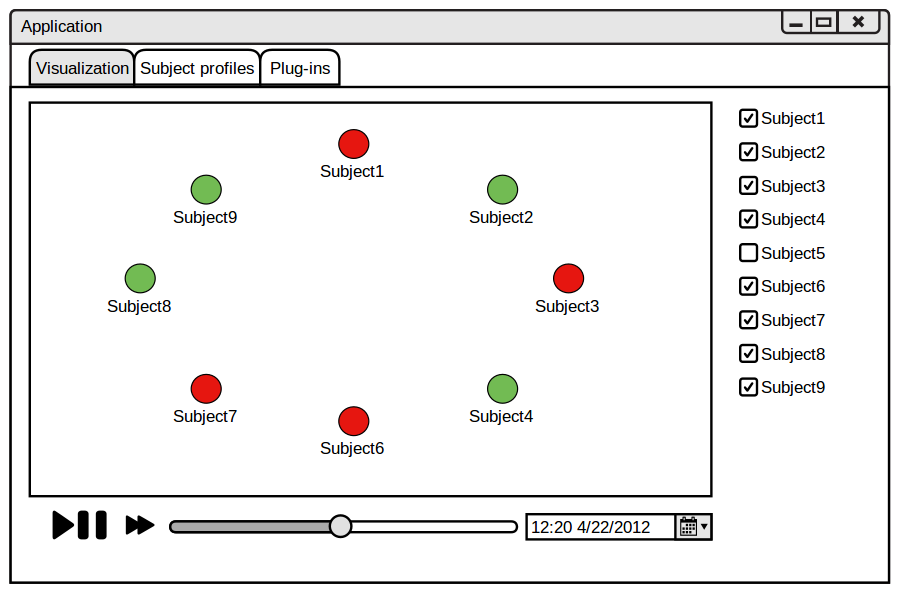
\includegraphics[width=1.0\textwidth]{./img/GUI/visualization.png}
	\end{center}
	\caption{GUI Scheme}\label{predstava}
\end{figure}

\section {Activities of the application} %<Files/Displayer-inside.jpg> // It should look like this, but the picture needs to have higher level, obviously
%\todo{TODO: pridat UML diagram akci}
%\section{Working with the application}
\paragraph{Selecting subjects}
Users should be able to select whatever subset of actions and subjects they want to replay in the animation of the case. After uploading the data, the application should generate names of all subjects and next to each one of them a check-box widget. Users should have the possibility to choose from them. Generally it would also be good to provide a possibility to choose a subset of all events directly from our database using a SQL query.

\paragraph{Adjusting the time period}
Under the animation frame there should be a scroll bar and a field indicating the corresponding time and date. Users should be able to move the scroll the bar below the animation frame manually and this way to travel in investigated period of time. At each point the corresponding scene should appear in the animation frame. The time should also be adjustable manually in the field that indicates corresponding time and date. After clicking the Play/Stop button replaying the visualization from this time further should start. 

\paragraph{Visualization}
After clicking on the button play/stop the animation of the scene should start replaying. The program will go through the database of events that the subjects did and for each event a spot representing the subject will change its color for a constant time period. If user stops (pauses) this playback and then starts it again the animation should continue from where it stopped. There should be a possibility to adjust the speed of replaying the case. 

\paragraph{Modes of replaying}
The application should provide two modes of replaying. First mode should be replaying according to the real time. Between every two events there should be the same proportion of time with regard to the time in reality. The purpose of this mode is to give the forensic auditor the idea of the time flow in the case. Second mode would serve as a quick replay of events. The period of time that has passed between every two events should be represented by a constant period of time in the visualization. The speed of time flow while replaying should be adjustable in both modes.

\paragraph{Subject activities}
The application should distinguish between several types of subject activities as shown in following overview.

%Activity | Example | Action
\begin{tabularx}{\textwidth}{l X}
Activity: & There is currently no Event involving this Subject.\\
Action: & The color of the dot representing the subject is red (Fig.\ref{subj_doing_nothing})\\
& 
\includegraphics[scale=0.3]{./img/visualization/subj_doing_nothing.png}\label{subj_doing_nothing}\\
\end{tabularx}\\

\begin{tabularx}{\textwidth}{l X}
%\hline
Activity: & Subject is doing something e.g. subject is causing an event\\
Example: & Subject4 is buying a new yacht. \\
Action: & The color of the dot representing the subject changes from red (no action) to green (indicating activity). After a globally adjustable time period the event the color of the dot changes back to red. If we have details about this event a small icon appears above the dot  revealing details of the event.\\ 
& 
\includegraphics[scale=0.3]{./img/visualization/subj_doing_sth.png}\\
\end{tabularx}\\

%\begin{figure}[h]
%	\begin{center} \label{subj_doing_sth}
%	
\includegraphics[]{./img/visualization/subj_doing_sth.png}
%	\end{center}
%	\caption{Activity of a subject}
%\end{figure}


\begin{tabularx}{\textwidth}{l X}
%\hline
Activity: & Subject is causing an event related to another subject. \\
Example: & Subject1 transfers some amount of money to Subject2's bank account.\\
Action: & The dot of the active subject changes color to green and a arrow from the active subject to the related one appears. After a globally adjustable time period the arrow disappears and the color of the dot changes back to red. If we have details about this event a small icon appears above the arrow. After clicking on it the icon reveals details of the event. \\
& 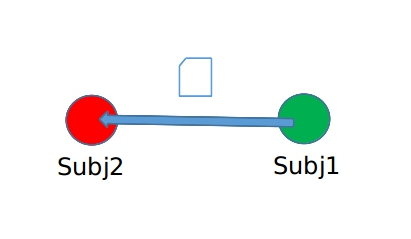
\includegraphics[scale=0.3]{./img/visualization/subj_sending_msg.png}\\


\end{tabularx}\\
\begin{tabularx}{\textwidth}{l X}
%\hline
Activity: & Several subjects are part of a event together. \\
Example: & Subject3, Subject6 and Subject7 have a business meeting together.\\
Action: & All dots representing corresponding subjects change color and a line connecting them together appears. After a globally adjustable time period all the dots are in default state (red color, no linking). If we have details about this event a small icon appears above the arrow. After clicking on it the icon reveals details of the event.\\
& 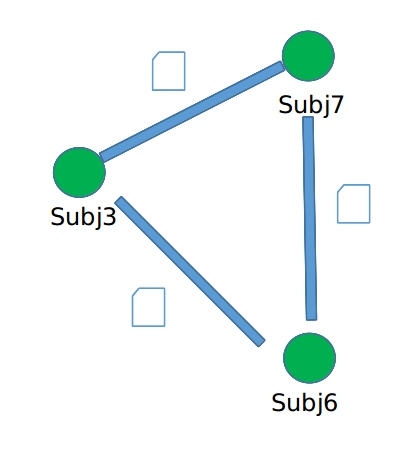
\includegraphics[scale=0.3]{./img/visualization/subjects_together.png}\\

\end{tabularx}



\section{Data}
The application should process data from very different sources. Since the application shall be used in last stages of forensic audit we expect that the data might be pre-selected by some quantitative or analytical software. Even though the application should not be limited by the amount of data, average usage is expected to work with the order of hundreds of events. Visualization of more events may not have the effect to help understand the situation. However, the application should be able to hold much more data in the database so that the forensic auditor could select form them.

Since there are many sources of data of different structure in forensic audit, our application is expected work as a superstructure with the purpose of the data projection only. The application should use data inserted to the application by various plug-ins. These plug-ins should transform the structure of data stored in the source (for example, instant messenger, email, accounting system, data from social networks etc.) to the data format used in our application. This two-layer division is chosen as it is easily expandable and universal. This project describes a standard interface for communication with these plug-ins.


Even though the implementation is not part of this project and the aim of this project is only to design the application, the design should be precise enough to make the implementation easy. 


\section{Example case}

The action of this application may be represented in following example case. Let us presume there is a company named "XYZ" where some money is missing. However, we are aware of those specific employees, of that certain enterprise, who have direct access to the company accounts. We also know the certain managers that are responsible for the company investments. Moreover, there are business partners of the company and also some regular employees such as workers. This case of money being disappeared has occurred during the period of 6 months. 

Forensic auditors receive the data from internal email, IM, telephone communication, from internal accounting system and is aware of the business operations of the company. They have also investigated information on the Internet on social sites. After accumulating all the data they use some analytical or quantitative software \ref{qSW} to discover the abnormalities in the accounting evidence. The rec SW recognize various connections between some of the subjects (common after work activities, common interests etc.). They have enough input, but still they need to find out what exactly happened. 

Forensic auditors decide to make use of our application for the investigative procedure. Firstly, they load all the outputs to the application and then they replay the events that happened during the last 6 months. Our system gives them an opportunity to deselect some subjects that seem to be irrelevant. They can also select the set of information for replaying via SQL query, i.e. the forensic auditor may arbitrarily replay those specific events that they demand. 




%To be able to design a new application 
%
%we need to make a series of decision and answer number of questions going from the most general to the most concrete. 
%Decisions and answers of the questions from the most general to the most concrete 
%
%All the decisions needed to be made to design the application are stated in the 


%\paragraph{Data format requirement} Our data will contain information of following structure: 
%every record of an action will contain ID of an record, name of the active subject, name(s) of 
%passive subject(s), the time of the action, and the record of remarks including details about 
%the action. These records will be stored in a database. We will be able to access all the 
%information. 
%
%
%\paragraph{Estimating the amount of data} We expect that our application will be used in final 
%stages of forensic audit, when we know the key period and only a few subjects remain. We expect 
%that we will be working with an order of hundreds of entries.






%\section{Working with the application}
%After uploading the data, the application should generate names of all subjects and for each one of them a check-box widget. This way users can select which subject they want in the animation of the case and which they want to displace in the next animation. 
%
%Below the animation frame there should be a scroll bar and a field indicating the corresponding time and date. Users should be able to move the scroll bar below the animation frame manually and this way to travel in investigated period of time. In each point a corresponding scene should appear in the animation frame. The time should also be adjustable manually in the field that indicates corresponding time and date. 
%
%User of this application should also have the possibility to select a subset of all events in the database using a SQL query. 
%
%After clicking on the button play/stop the animation of the scene should start replaying.The program will go through the database of events that the subjects did and for each event a spot representing the subject will change its color for an adjustable period.  If user stops (pauses) this playback and then starts it again the animation should continue. There should be a possibility to adjust the speed of replaying the case. 

%\subsection{GUI requirements} 
%We have decided that the user interface of our program will look 
%as follows. The main part of the area will be the middle panel. We want this panel to contain 
%one spot for each subject of our case. These spots will be in a circle by default. This will be 
%the part of visualization that will help understand the sequence of events. 
%
%There will be a time axis under this panel with a slider and play and stop buttons. After 
%clicking the play button, the main action of this application will start. The program will go 
%through the database of events that the subjects did and for each event a spot representing the 
%subject will change its color for an adjustable period. 

%\todo{TODO: pridat obrazek priblizneho vysledku}


 
%\chapter*{Design}
%% !TeX spellcheck = en_US
%\chapter{Design} 
%\section{Design of the data access}
%\section{Filters}

%=======================================================================
\chapter{Design of an information system for support of forensic audit}\label {Design}
%\komentar{
%vsechno o tom systemu jako takovem, ale tak, aby to navazovalo na predchozi...?
%
%prostredi webu + silne zabezpeceni, reporty, export, pdf\\
%maly informativni obrazek, ktery poskytne uzivateli informaci o tom, co se stalo\\
%! pripojit pripady uziti vcetne zavislosti\\
%
%jedna se o aplikaci, ktera provazi celym projektem (zadanim) forenzniho auditu. sice existuji i jiny nastroje pro podporu takovychto projektu, ale projekt ma useky a nam jde o integraci porizenych vysledku
%
%}

%=======================================================================

This chapter deals with the design of the information system. Approaches to the implementation of requirements on the system stated in \ref{Requirements} are described here. We also provide a discussion about technologies useful for implementation and the description is accompanied with diagrams demonstrating the design. 

\section{Application}

The architecture of our application will be based on two fundamental parts. One of them will be collecting the data we will use and the other will display them to the user. From now on we will call this the \name{Collector} and the \name{Displayer}. This is a useful division because it simplifies the design and also keeps it easier to maintain. The aim of the \name{Collector} will be to transform the data from various sources to some generic format for easier manipulation.

There are numerous types of sources of data that can be used as evidence in forensic audit. The data can differ in inner structure and also in the content. Examples of this diversity are IM messages, pictures, GPS coordinates, audio-video files,emails logs of network activities, public information from social sites and internal company management or accounting system.

Ideally our system is able to work with all of them, however we exclude pictures and the audio-video material from these sources because this material does not need visualization. Nevertheless, our system needs to be able to process the information this type of material contains, in case that it could be converted to the basic structure of our application, which will be described later. The task to provide this functionality is assigned to the \name{Collector}.

Each of the previously mentioned type of source of data is somehow specific. Thus we need a specific solution for each one of them. This is an ideal job for a plug-in architecture. 

\begin{figure}[!h]
    \centering 
    \epsfysize=60mm 
    \epsffile{./img/diagrams/Architecture.eps} 
    \caption{Architecture of the application}\label{Architecture}
\end{figure}

Plug-in is a piece of software that does not work separately, it only extends the functionality of the application. The application usually provides an Application Programming Interface (API) so that the plug-in extension could communicate with the application properly. In case of this application it means that for each source of data there will be a specific plug-in. each plug-in will be made specifically for the format of the source file. The purpose of the plug-in will be to read the source files and prepare the data for the \name{Collector}. The collector than saves it to the database. Finally the \name{Displayer} will access the database and provide the visualization of the case.

\begin{figure}[!h]
    \centering 
    \epsfysize=60mm 
    \epsffile{./img/diagrams/Plug-ins.eps} 
    \caption{Collector}\label{Collector}
\end{figure}

\subsection{Database}
\paragraph{Entity \name{Event}}
The database model of our application is based on a entity called \name{Event} and several other entities. The Primary unique identification number (UID) of \name{Event} is Integer ID. It also consists of one mandatory time-stamp that indicates the time this event occurred or the time of the start if the event was long-lasting. We need to distinguish between one-time events and longer lasting ones so in there is a mandatory boolean attribute \name{LongLasting} playing the role of a flag. If this attribute is true, another time-stamp attribute indicating the end of the \name{Event} is to be filled in. 

\begin{figure}[!h]
    \centering 
    \epsfysize=180mm 
    \epsffile{./img/datamodel/logical.pdf} 
    \caption{Logical model of the database}\label{Logical}
\end{figure}

\paragraph{Entity \name{Event\_Detail}}
We have prepared a entity \name{Event\_Detail} in case there would be some other details concerning the \name{Event}. This entity is in a 1:n relationship with \name{Event}. It means, that if we will need, there can be more details concerning \name{Event}. \name{Event\_Detail} has only one mandatory attribute called \name{Description}, that is prepared for 128 characters of text. For \name{Event} the relationship with \name{Event\_Detail} is optional, however, for \name{Event\_Detail} it is compulsory and the ID of \name{Event} is its foreign key. 

\paragraph{}
The data we expect to use as a source should also contain information about the subject causing the event. For the subject we have a special model. Before describing it, let us explain why we need it. We cannot be sure what sources and what information concerning the subjects we will get. Our source files should primarily contain logs of various kinds of activities, not only logs of one subject. Because of this we cannot easily connect actual person with events. The identifier of the subject can be of different kind in different sources. For example while email clients are identified by email address, e.g. character stings, IM users are identified by integer ID, nickname or even e-mail address. However this identifier is definitely not the same as the bank account number. Still ne subject may be identified by any number of any of these ways.

For simplicity we decided not to deal with merging these various accounts of one subject in the database as it would increase complexity greatly. This will be done later by the \name{Displayer}. 

\paragraph{\name{Participant}}
In our database model we now establish the \name{Participant} entity. The primary key of this entity is an integer ID and next attribute is optional a 36-char-long \name{Name}. This attribute is prepared for the case that the name of the participant would be stated in the source. For actual information about the source we prepare two extra mandatory attributes. The first, called \name{type}, is designed to inform about the source of data the particular information came from. The second one is called \name{alias} and it is an array of 32 characters prepared to store the original identifier of the participant.

The \name{Participant} entity contains two other entities called \name{Active} and \name{Passive}. Each one of them has the entity \name{Participant} as its superstructure. The relationship between \name{Participant} and \name{Event} is arranged via these two entities. Both these relationships are of m:n type. The only difference between them is that  for the \name{Event} entity the relationship with \name{Active Participant} is compulsory whereas with \name{Passive Participant} is optional. 

This model enables \name{Events} to have more \name{Participants}, but forces the \name{Event} to have at least one \name{Active Participant}.


\begin{figure}[!h]
    \centering 
    
    \epsfysize=180mm 
    \epsffile{./img/datamodel/relational.pdf} 
    \caption{Relational model}\label{Relational}
\end{figure}

\subsection{\name{Collector}} 

The next section focuses on the \name{Collector} part of the application. Before we start let us mention that the main purpose of the \name{Collector} is to provide an interface for inserting data to the database and managing the plug-ins that translate the source format to our format (based on the event structure). The \name{Collector} has its own GUI that enables the user to choose from existing plug-ins or add new ones. The GUI saves the configuration to a configuration file and then hands it over to the \name{Collector} back end. The \name{Collector} provides the user the possibility of selecting and running the plug-ins. Each plug-in has its own GUI so that the user can specify any information needed for them to run of the plug-in (such as the path to a file with the source material). 

The \name{Collector} also manages the plug-ins added to the application. It means that it has a configuration file where all paths to the plug-ins are saved together with short clear description of the source. %\todo{} (tady jsem nejak prestala) \todo{}

The key API that the \name{Collector} provides to the plug-in is basically the access to the database. %It might be a bit risky to provide the access to the database to a unknown piece of software.
Plug-ins load data into the tables and the \name{Collector} pushes the data into the database. Each plug-in only processes the source file to the data model, create a SQL query and fill in the database. Note, that this application is expected to process data of a text character only. The application is not prepared for mining data from files of multimedia character unless the content is described in a structured text containing the date and some information identifying the related subject.

\begin{figure}[h]
	\begin{center} 
	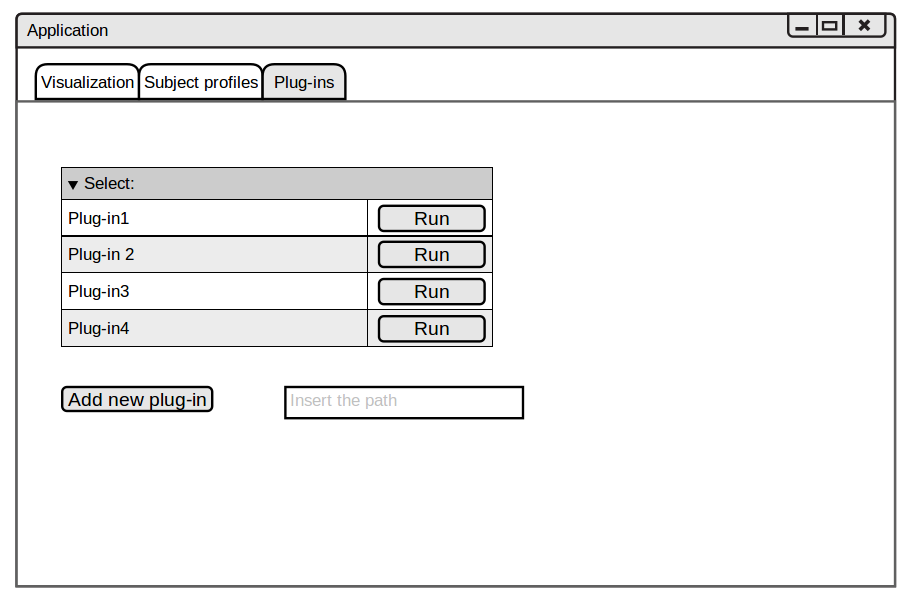
\includegraphics[width=1.0\textwidth]{./img/GUI/Plug-ins.png}
	\end{center}
	\caption{Graphical user interface of the plug-in manager}\label{plug-ins}
\end{figure}

\subsection{\name{Displayer}}

The main purpose of the displayer is to visualize the data saved in the database. To be able to do this, it is necessary at first to deal with the problem of multiple \name{Participants} in the database that all represent the same \name{Subject}. We can overcame this obstacle easily by creating a table for \name{Participant} unification to \name {Subjects}. However, because of the essence of the data we are working with and the general purpose of our application, we cannot try to guess which \name{Participants} belong together. Therefore there is a special form helping the auditor unify them to subjects. 

\begin{figure}[h]
	\begin{center} 
	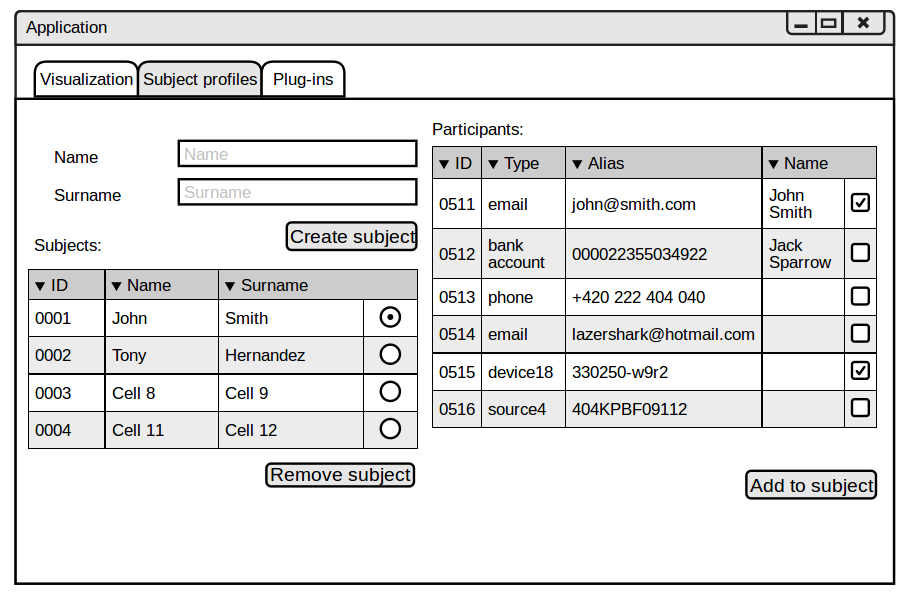
\includegraphics[width=1.0\textwidth]{./img/GUI/Subject_profiles.png}
	\end{center}
	\caption{Form for unifying \name{Participants} to Subjects}\label{form}
\end{figure}

Sample form is shown in the figure \ref{form}. In the left table there is a list of existing subjects. The user can add new subjects easily by filling in the name and surname and by clicking on the "Create subject" button. Auditor can also remove a subject by clicking on "Remove subject" button or edit name or surname of subject by clicking into the table. The \name{Displayer} creates a table containing the information about this mapping. When replaying the displayer uses this information to identify the correct events for each subject. The data model shown in picture \ref{model-displayer} indicates that each \name{Subject} can have many \name{Participants}, but each \name{Participant} can have only one \name{Participant}.

\begin{figure}[!h]
    \centering 
    
    \epsfysize=40mm 
    \epsffile{./img/datamodel/subj-participant.pdf} 
    \caption{The relation between \name{Subject} and \name{Participant}}\label{model-displayer}
\end{figure}

Now we can focus on the most important function of the application. We have a background for the visualization in the above modeled database. In the initialization phase the \name{Displayer} generates names of all the known \name{Subjects} and places a checkbox next to each one of them. The state of the checkbox decides whether we want to include the related \name{Subject} in the visualization. 

In the next step the \name{Displayer} enters proper SQL query. IDs of the subjects are replaced by the entire group of \name{Participants}. We then search in the database for all \name{Events} whose starting time is later than the date selected in the visualization tab and at the same time the some of the \name{Subjects} takes part in it. We also search for  \name{LongLasting} \name{Events} that end after the selected time frame. The result of the  selected  \name{Events} is then replayed by time. 

The process of replaying has a small obstacle concerning various animations in different cases. These differences are:
\begin{enumerate}
\item If \name{Subject} does not take part in current \name{Event} it is displayed as a red dot.
\item If \name{Subject} takes part in a \name{Event} alone it is displayed as a green dot.
\item If \name{Subject} causes an \name{Event} the color of the active \name{Subject} is green and a arrow aiming at the passive \name{Subject} is displayed. 
\item If more \name{Subjects} actively participate in one \name{Event} they are all displayed in green color and a line connecting them together is displayed between them. 
\end{enumerate}

 The solution for the first and second case is trivial. The color of all \name{Subjects} is red by default so only if we run into a \name{Event} where a subject takes a part we change the color for a constant period of displayed time. If the \name{Event} has a passive \name{Participant}, as described in third case, we draw an arrow from the active to the passive \name{Subject}. Similarly, if the \name{Event} has more \name{Active Participants} the line between them is drawn.  
 
 All these situations are easily recognizable using SQL queries. 
% 
% 
%\todo{} The inner design of the \name{Displayer}
%It was already mentioned that the \name{Displayer} acquires \name{Events} for replaying using SQL queries. There is only one aspect left to describe and it is the inner design of the \name{Displayer}. To be able to run the \name{Displayer} needs the table mapping  \name{Participants} to \name{Subjects}. We recommend not to save this table in the database, but rather store it in memory for faster accessibility. The user needs to follow only several units of subjects in the animation. \todo
% 
 
 
\chapter{Discussion} \label{Discussion}

%popis rozdil mezi flatfile a databazi externi vs embeded
\paragraph{Database} %\todo{}

We recommend to use the Oracle database. The main reason is that it is one of the fastest and safest relational databases. If it was necessary since it is a relational database it could be replaced for any other relational database and the Oracle Data Modeler is also very easy to use, we have already some good experience with it. 

\paragraph{Open Database Connectivity}
Open Database Connectivity (ODBC) is a standardized software API that enables the access to database servers. The aim of ODBC is to provide an access independent on programming language, operating system or the database system. We recommend to use this technique while implementing this application. 

We would also recommend to use the C/C++ programming language. The Qt library can be used for implementation of the GUI of this program.

\paragraph*{Further improvement}
Follow-up work would definitely include the implementation of the designed application, testing and hands-on experience with real data.
Mainly real-world use will show deficiencies, if any, and provide necessary insight for modifications and extensions.


%paragraph{Flat File} 
%
% flat file database is the simplest form of database. It stores data in a plain text file \cite{x2}.%http://techterms.com/definition/flatfile 
%here is one record per line. Fields in each line are separated by 
%elimiters such as tabulator or comma. In this model data are stored in multiple files, however these 
%iles are not linked, so the data may be repeated in several files. The advantage of this kind of database is the simplicity.
%t can also be easily transformed into most other databases. One disadvantage is performance drop for large databases, which may 
%equire linear walk for random access, thus loading unnecessary data into memory. Another disadvantage is 
%hat a flat file usually requires writing and debugging custom code, which may extend the time to develop the application.
%t is not a widely used type of a database. 
%
%
%paragraph{SQL database management system}
%oday's SQL databases provide reliable data storage with the widest feature sets, powering some of the biggest companies.Their advantages include large feature sets and independence on the applications that use them and they are well documented and easy to first setup thanks to them being so commonplace
%n the other hand they are criticized for their lack of performance, bloated specifications and difficult optimizations which are required when their aforementioned lack
%f performance shows itself.
%
%xamples include MySQL, PostgreSQL and IBM DB2.
%
%paragraph{NoSQL database} %<-tohle je nejrychlejsi
%
%oSQL databases handle data based on different models than relational databases. Their data model is more tightly coupled with the needs of the application.
%hese databases may or may not use general query language to access data (NoSQL may be also interpreted as Not-only-SQL), but they particularly shine when they don't and instead the application uses their API
%o access the data directly.
%
%heir performance is often unmatched, but may be more difficult to use due to their lack of powerful tools the SQL offers.
%
%here are several methods to categorize NoSQL databases, all with diverse classes and subclasses. Because of the variability of the methodologies and overlays it is problematic to acquire and preserve an indication of non-relational databases. Yet, a basic arrangement is based on data model. A few examples in each group are:
%
%begin{itemize}
%item \textbf{Graph:} InfiniteGraph, OrientDB
%item \textbf{Multi-model:} ArangoDB, Alchemy Database
%item \textbf{Column:} Druid, Hbase
%item \textbf{Document:} Clusterpoint, OrientDB
%item \textbf{Key-value:} Oracle NoSQL Database, Dynamo, LMDB, LevelDB
%end{itemize}
%
%
%paragraph{NewSQL database} %<-tohle by asi bylo idealni
%he NewSQL database is a type of modern relational database management system that attempts to combine the speed and efficiency of NoSQL databases while 
%etaining the relational database model.
%
%mong NewSQL databases may be included these: H-Store, Clustrix, VoltDB, MemSQL.
%
%he NewSQL database will be more appropriate for storing our data in terms of its speediness and functionality for forensic investigation, as compared to the rest of the database techniques mentioned above. Especially more complex operations on data would be missed on databases without SQL support.
%
%
%








 %\addcontentsline{toc}{chapter}{Design}
%\chapter*{Conclusion} 
\addcontentsline{toc}{chapter}{Conclusion}   % SEM NESAHEJTE!
%\chapter*{Conclusion} \label{Conclusion}

The aim of this bachelor project was to design an information system for support of forensic audit. 
This bachelor project describes the whole process of forensic audit and analyses the software used in the 
process and methods of the audit that could be supported by a new application. A method of this kind 
was found and an information system designed. One part of the design is an analysis that describes 
possible approaches of the design and the consequences of the decisions for each one of them. The choice 
of the final design was reasoned and properly described. The discussion of the technologies to be used 
for the implementation is provided. There is minimum of questions left do answer for 
implementing this application. 


%\section*{Accomplishment} 

It can be said the main aim has been accomplished. The application supporting 
the one part of the process of forensic audit is designed. All main decisions for the functioning of 
the application has been made and a good background for implementation of the application is provided. 
After the implementation and testing the application will be prepared to be used in practice. 



%\section*{Further improvement}
%Follow-up work would definitely include the implementation of the designed application, testing and hands-on experience with real-data.
%Mainly real-world use will show deficiencies, if any, and provide necessary insight for modifications and extensions.
%
  % Závěr, je vkládán z jiného souboru









%%%%%%%%%%%%%%%%%%%%%%  Seznam použitých zdrojů  %%%%%%%%%%%%%%%%%%%%%%
\newpage  % SEM NESAHEJTE!
\renewcommand{\bibname}{Bibliography} % SEM NESAHEJTE!
\addcontentsline{toc}{chapter}{Bibliography} % SEM NESAHEJTE!Seznam použitých zdrojů

% !!! Literatura se řadí abecedně.
%\input{vnitrek_literatura.tex}  % text, který je vkládán z jiného souboru, MŮŽETE ZMĚNIT NÁZEV souboru nebo smazat tento řádek a seznam literatury napsat přímo sem

\bibliographystyle{plain}
\bibliography{literatura}



\newpage % SEM NESAHEJTE!
%%%%%%%%%%%%%%%%%%%%%%  PŘÍLOHY PRÁCE %%%%%%%%%%%%%%%%%%%%%%
%\appendix  % přílohy budou opravdu "Přílohy"  :-)     SEM NESAHEJTE!
%\addcontentsline{toc}{chapter}{Attachment} % přidat položku do obsahu      SEM NESAHEJTE!

%\part*{Attachment}  % SEM NESAHEJTE!
\chapter*{Attachment A}
\addcontentsline{toc}{chapter}{Attachment A}

\section*{Contents of the CD}
\addcontentsline{toc}{section}{Contents of the CD}

\subsection*{The text of this bachelor project in pdf}
The text of this bachelor project is saved as \verb-BP_Peskova.pdf- in root folder. 

\renewcommand{\appendixname}{Attachment} % aby se přílohy nejmenovaly "Dodatek"  SEM NESAHEJTE!

%-------- zde VYMĚŇTE NÁZVY vkládaných souborů NEBO sem můžete rovnou napsat text příloh (a smažte dva následující řádky)
%\input{vnitrek_priloha1.tex} % příloha 1: vložená z externího souboru
%\input{vnitrek_priloha2.tex} % příloha 2: vložená z externího souboru

\end{document} % SEM NESAHEJTE!
